\documentclass{article}
\usepackage{ctex}
\usepackage{geometry}
\geometry{a4paper, scale=0.8}
\usepackage{graphicx}
\usepackage{float}
\usepackage{enumitem}
\usepackage{amsmath}
\usepackage{amssymb}

\title{银行业务管理系统数据库设计 \\ {\small 数据库实验二报告}}
\author{PB19071405 \ 王昊元}
\date{2022 年 04 月 30 日}

\begin{document}
    \maketitle

    \section{概念模型设计}
    \subsection{实体设计}
    \begin{itemize}
        \item ``银行有多个支行。各个支行位于某个城市,每个支行有唯一的名字。银行要监控每个支行的资产。'': \\
        支行实体包括它的名称、所在城市和资产。
        \item ``银行的客户通过其身份证号来标识。银行存储每个客户的姓名、联系电话以及家庭住址。为了安全起见,银行还要求客户提供一位联系人的信息,包括联系人姓名、手机号、Email以及与客户的关系。'': \\
        客户实体包括身份证号、姓名、联系电话、家庭住址、联系人的信息(姓名、手机号、Email和关系)。
        \item ``银行员工也通过身份证号来标识。员工分为部门经理和普通员工。''、``银行还需知道每个员工开始工作的日期。''、``每个支行的管理机构存储每个员工的姓名、电话号码、家庭地址、所在的部门号、部门名称、部门类型及部门经理的身份证号。'': \\
        员工实体包括身份证号、姓名、电话号码、家庭住址、入职时间。部门实体包括部门号、部门名称、部门类型。部门经理为员工的子类实体。
        \item ``银行提供两类帐户——储蓄帐户和支票帐户。''、``每个帐户被赋以唯一的帐户号。银行记录每个帐户的余额、开户日期、开户的支行名以及每个帐户所有者访问该帐户的最近日期。''、``每个储 蓄帐户有利率和货币类型,且每个支票帐户有透支额。'': \\
        账户实体中值包括账户号、余额、开户日期、最近访问日期。储蓄账户实体和支票账户实体是账户的子类实体。储蓄账户实体还包括利率和货币类型,支票账户实体还包括透支额。
        \item ``每笔贷款用唯一的贷款号标识。银行需要知道每笔贷款所贷金额以及逐次支付的情况(银行将贷款分几次付给客户)。虽然贷款号不能唯一标识银行所有为贷款所付的款项,但可以唯一标识为某贷款所付的款项。对每次的付款需要记录日期和金额。'': \\
        贷款部分设计两个实体,贷款实体与支付实体。贷款实体包括贷款码和贷款金额。支付实体包括支付码、日期和金额。
    \end{itemize}
    \subsection{联系设计}
    \begin{itemize}

        \item ``每个部门经理都负责领导其所在部门的员工,并且每个员工只允许在一个部门内工作。'': \\
        支行设立部门,部门经理管理部门,员工隶属于部门。
        \item ``客户可能和某个银行员工发生联系,该员工是此客户的贷款负责人或银行帐户负责人。'': \\
        员工负责着客户,有着不同的负责类型。
        \item ``帐户可以由多个客户所共有,一个客户也可开设多个账户,但在一个支行内最多只能开设一个储蓄账户和一个支票账户。'': \\
        客户持有着账户。而客户在一个支行内最多只能开设一个储蓄账户和一个支票账户,也就是说客户对于一个支行来说,``储蓄账户持有''和``支票账户持有''的联系最多存在一个。
        而``帐户可以由多个客户所共有''则通过不约束进行实现,例如多个客户的持有关系指向同一个账户,即代表该账户由多个客户持有。
        \item 支行开设账户。
    \end{itemize}
    \subsection{Power Design 的 ER 图}
    \begin{figure}[H]
        \centering
        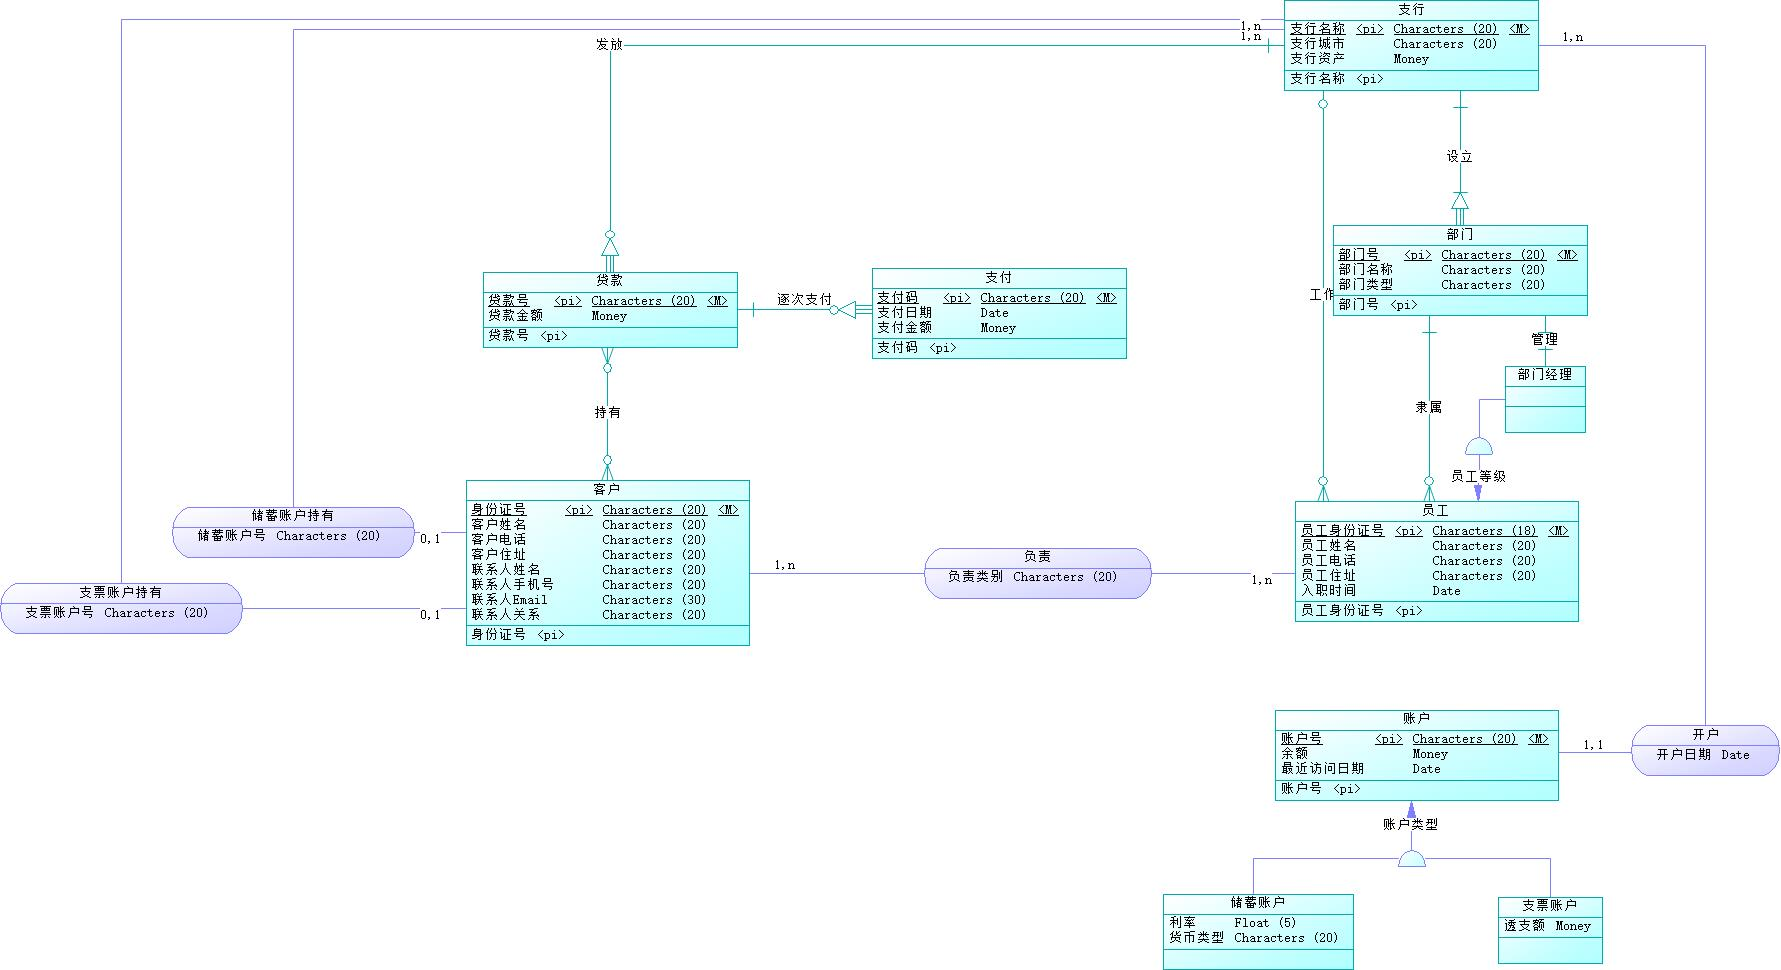
\includegraphics[width=0.8\textwidth]{./lab02/cdm.jpg}
        \caption{Power Design 的 ER 图}
    \end{figure}
    \section{概念模型到逻辑模型的转换}
    \subsection{实体转换}
    \begin{itemize}
        \item 将实体转换为关系模式,实体的属性为关系模式的属性,实体的标识成为关系模式的主码。
        \item 在子类关系模式中加入父类的主码,子类关系模式的主码设为父类的主码。如员工是父类,部门经理是子类,账户是父类,两种具体的账户类型是子类。
    \end{itemize}
    \subsection{联系转换}
    \begin{itemize}
        \item 员工与支行的联系为1:N,则将支行名称加入员工关系模式中,类似的还有员工与部门之间、账户与支行之间、账户持有联系等等。
        \item 客户和贷款之间的关系为M:N,则新建一个``持有''关系模式,连接客户和贷款。
    \end{itemize}
    \subsection{最终的关系模式}
    \begin{figure}[H]
        \centering
        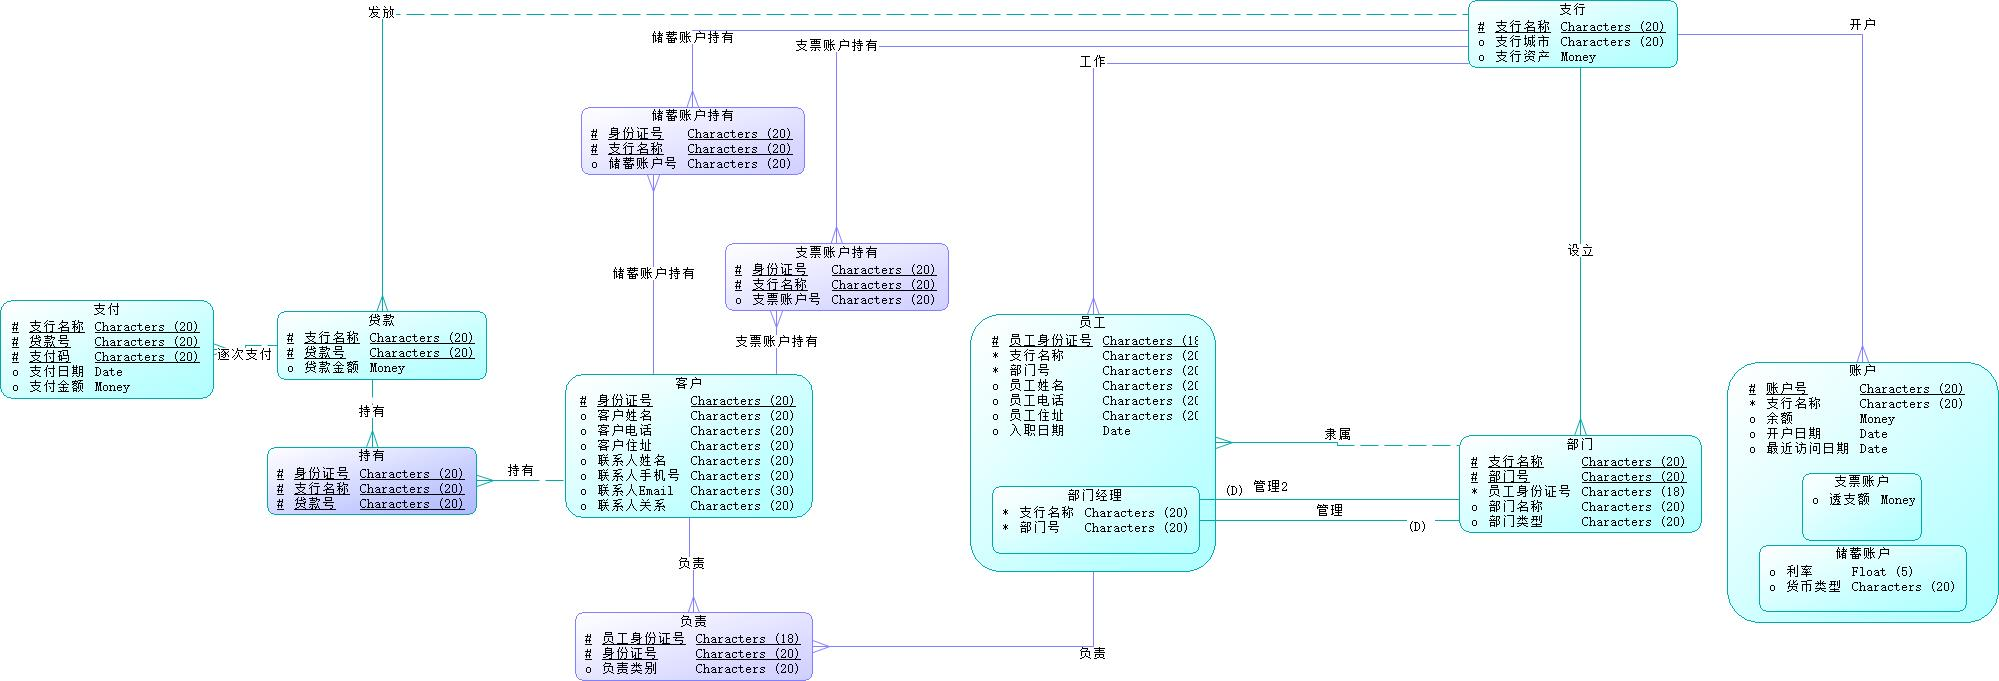
\includegraphics[width=0.8\textwidth]{./lab02/ldm.jpg}
        \caption{最终的关系模式}
    \end{figure}
    \section{MySQL数据库结构实现}
    \subsection{Power Design PDM图}
    \begin{figure}[H]
        \centering
        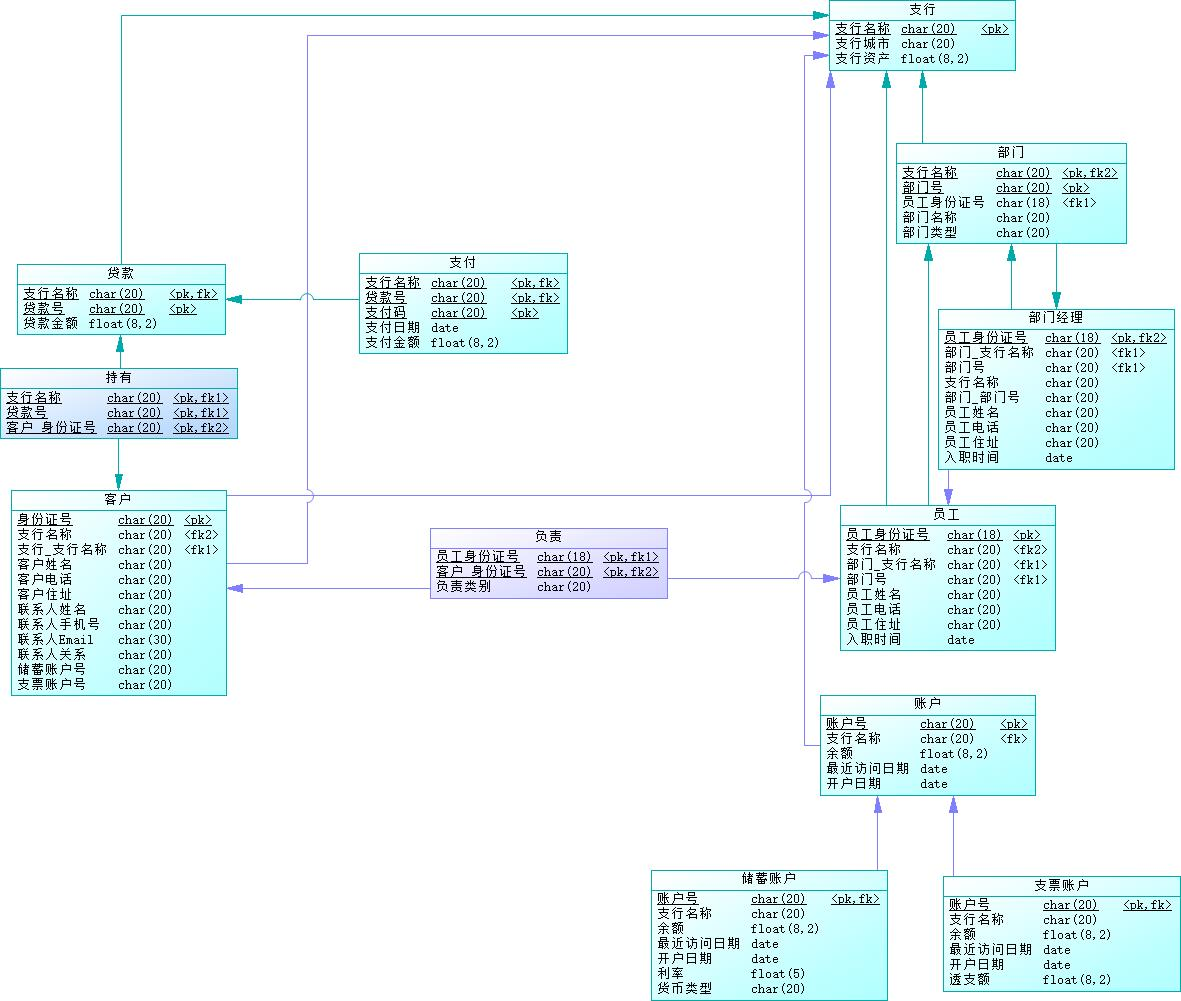
\includegraphics[width=0.8\textwidth]{./lab02/pdm.jpg}
        \caption{Power Design PDM图}
    \end{figure}
    \subsection{数据库表定义}
    \begin{table}[H]
        \centering
        \caption{支行表\ subbank}
        \begin{tabular}{cccccc}
            \hline
            列名 & 中文含义 & 类型 & 允许为空 & 是否主键 & 是否外键 \\
            \hline
            name & 支行名称 & char(20) & 否 & 是 & 否 \\
            city & 支行城市 & char(20) & 是 & 否 & 否 \\
            property & 支行资产 & float & 是 否 & 否 \\
            \hline
        \end{tabular}
    \end{table}
    \begin{table}[H]
        \centering
        \caption{部门表\ department}
        \begin{tabular}{cccccc}
            \hline
            列名 & 中文含义 & 类型 & 允许为空 & 是否主键 & 是否外键 \\
            \hline
            subbank\_name & 支行名称 & char(10) & 否 & 是 & 是(subbank) \\
            id & 部门号 & char(20) & 否 & 是 & 否 \\
            manager\_id & 部门经理身份证号 & char(18) & 是 & 否 & 是(department\_manager) \\
            name & 部门名称 & char(20) & 是 & 否 & 否 \\
            type & 部门类型 & char(20) & 是 & 否 & 否 \\
            \hline
        \end{tabular}
    \end{table}
    \begin{table}[H]
        \centering
        \caption{员工表\ employee}
        \begin{tabular}{cccccc}
            \hline
            列名 & 中文含义 & 类型 & 允许为空 & 是否主键 & 是否外键 \\
            \hline
            id & 员工身份证号 & char(18) & 否 & 是 & 否 \\
            subbank\_name & 支行名称 & char(20) & 是 & 否 & 是(subbank) \\
            department\_subbank\_name & 部门\_支行名称 & char(20) & 是 & 否 & 是(department) \\
            department\_id & 部门号 & char(20) & 是 & 否 & 是(department) \\
            name & 员工姓名 & char(20) & 是 & 否 & 否 \\
            phone & 员工电话 & char(20) & 是 & 否 & 否 \\
            addr & 员工住址 & char(20) & 是 & 否 & 否 \\
            start\_date & 入职时间 & date & 是 & 否 & 否 \\
            \hline
        \end{tabular}
    \end{table}
    \begin{table}[H]
        \centering
        \caption{部门经理表\ department\_manager}
        \begin{tabular}{cccccc}
            \hline
            列名 & 中文含义 & 类型 & 允许为空 & 是否主键 & 是否外键 \\
            \hline
            id & 部门经理身份证号 & char(18) & 否 & 是 & 否 \\
            department\_subbank\_name & 部门\_支行名称 & char(20) & 是 & 否 & 是(department) \\
            department\_id & 部门号 & char(20) & 是 & 否 & 是(department) \\
            subbank\_name & 支行名称 & char(20) & 是 & 否 & 是(subbank) \\
            lead\_department\_id & 领导的部门号 & 是 & 否 & 是(department) \\
            name & 部门经理姓名 & char(20) & 是 & 否 & 否 \\
            phone & 部门经理电话 & char(20) & 是 & 否 & 否 \\
            addr & 部门经理住址 & char(20) & 是 & 否 & 否 \\
            start\_date & 入职时间 & date & 是 & 否 & 否 \\
            \hline
        \end{tabular}
    \end{table}
    \begin{table}[H]
        \centering
        \caption{账户表\ account}
        \begin{tabular}{cccccc}
            \hline
            列名 & 中文含义 & 类型 & 允许为空 & 是否主键 & 是否外键 \\
            \hline
            id & 账户名 & char(20) & 否 & 是 & 否 \\
            subbank\_name & 支行名称 & char(20) & 是 & 否 & 是(subbank) \\
            balance & 余额 & float & 是 & 否 & 否 \\
            recent\_date & 最近访问日期 & date & 是 & 否 & 否 \\
            open\_date & 开户日期 & date & 是 & 否 & 否 \\
            \hline
        \end{tabular}
    \end{table}
    \begin{table}[H]
        \centering
        \caption{储蓄账户表\ deposit\_account}
        \begin{tabular}{cccccc}
            \hline
            列名 & 中文含义 & 类型 & 允许为空 & 是否主键 & 是否外键 \\
            \hline
            id & 账户名 & char(20) & 否 & 是 & 否 \\
            subbank\_name & 支行名称 & char(20) & 是 & 否 & 是(subbank) \\
            balance & 余额 & float & 是 & 否 & 否 \\
            recent\_date & 最近访问日期 & date & 是 & 否 & 否 \\
            open\_date & 开户日期 & date & 是 & 否 & 否 \\
            rate & 利率 & float & 是 & 否 & 否 \\
            money\_type & 货币类型 & char(20) & 是 & 否 & 否 \\
            \hline
        \end{tabular}
    \end{table}
    \begin{table}[H]
        \centering
        \caption{支票账户表\ cheque\_account}
        \begin{tabular}{cccccc}
            \hline
            列名 & 中文含义 & 类型 & 允许为空 & 是否主键 & 是否外键 \\
            \hline
            id & 账户名 & char(20) & 否 & 是 & 否 \\
            subbank\_name & 支行名称 & char(20) & 是 & 否 & 是(subbank) \\
            balance & 余额 & float & 是 & 否 & 否 \\
            recent\_date & 最近访问日期 & date & 是 & 否 & 否 \\
            open\_date & 开户日期 & date & 是 & 否 & 否 \\
            overdraft & 透支额 & float & 是 & 否 & 否 \\
            \hline
        \end{tabular}
    \end{table}
    \begin{table}[H]
        \centering
        \caption{客户表\ client}
        \begin{tabular}{cccccc}
            \hline
            列名 & 中文含义 & 类型 & 允许为空 & 是否主键 & 是否外键 \\
            \hline
            id & 身份证号 & char(18) & 否 & 是 & 否 \\
            loan\_subbank\_name & 贷款支行名称 & char(20) & 是 & 否 & 是(subbank) \\
            subbank\_name & 账户所在支行名称 & char(20) & 是 & 否 & 是(subbank) \\
            name & 客户姓名 & char(20) & 是 & 否 & 否 \\
            phone & 客户电话 & char(20) & 是 & 否 & 否 \\
            addr & 客户住址 & char(20) & 是 & 否 & 否 \\
            link\_name & 联系人姓名 & char(20) & 是 & 否 & 否 \\
            link\_phone & 联系人手机号 & char(20) & 是 & 否 & 否 \\
            link\_email & 联系人Email & char(20) & 是 & 否 & 否 \\
            relationship & 联系人关系 & char(20) & 是 & 否 & 否 \\
            deposit\_account\_id & 储蓄账户号 & char(20) & 是 & 否 & 是(deposit\_account) \\
            cheque\_account\_id & 支票账户号 & char(20) & 是 & 否 & 是(cheque\_account) \\
            \hline
        \end{tabular}
    \end{table}
    \begin{table}[H]
        \centering
        \caption{贷款表\ loan}
        \begin{tabular}{cccccc}
            \hline
            列名 & 中文含义 & 类型 & 允许为空 & 是否主键 & 是否外键 \\
            \hline
            subbank\_name & 支行名称 & char(20) & 否 & 是 & 是(subbank) \\
            id & 贷款号 & char(20) & 否 & 是 & 否 \\
            money & 贷款金额 & float & 是 & 否 & 否 \\
            \hline
        \end{tabular}
    \end{table}
    \begin{table}[H]
        \centering
        \caption{支付表\ payment}
        \begin{tabular}{cccccc}
            \hline
            列名 & 中文含义 & 类型 & 允许为空 & 是否主键 & 是否外键 \\
            \hline
            subbank\_name & 支行名称 & char(20) & 否 & 是 & 是(subbank) \\
            loan\_id & 贷款号 & char(20) & 否 & 是 & 是(loan) \\
            id & 支付码 & char(20) & 否 & 是 & 否 \\
            payment\_date & 支付日期 & date & 是 & 否 & 否 \\
            payment\_money & 支付金额 & float & 是 & 否 & 否 \\
            \hline
        \end{tabular}
    \end{table}
    \begin{table}[H]
        \centering
        \caption{负责表\ response}
        \begin{tabular}{cccccc}
            \hline
            列名 & 中文含义 & 类型 & 允许为空 & 是否主键 & 是否外键 \\
            \hline
            employee\_id & 员工身份证号 & char(18) & 否 & 是 & 是(employee) \\
            client\_id & 客户身份证号 & char(18) & 否 & 是 & 是(client) \\
            response\_type & 负责类型 & char(20) & 是 & 否 & 否 \\
            \hline
        \end{tabular}
    \end{table}
    \begin{table}[H]
        \centering
        \caption{持有表\ own}
        \begin{tabular}{cccccc}
            \hline
            列名 & 中文含义 & 类型 & 允许为空 & 是否主键 & 是否外键 \\
            \hline
            subbank\_name & 支行名称 & char(20) & 否 & 是 & 是(subbank) \\
            loan\_id & 贷款号 & char(20) & 否 & 是 & 是(loan) \\
            client\_id & 客户身份证号 & char(18) & 否 & 是 & 是(client) \\
            \hline
        \end{tabular}
    \end{table}
    
    \section{总结与体会}
    \begin{enumerate}[label=\arabic*.]
        \item 体会到了Power Designer的强大和做数据库模式设计的必要性,也感受到了数据库逻辑的缜密。
        \item 在自己做设计,能感受到自己设计经验的不足,很多地方逻辑设计得不够清晰与简洁,
        可能会导致实现时的不便。
        \item 在设计和总结的过程中,能发现自己的设计中还存在着冗余的设计或者属性,
        在许多细节上设计得也不是很到位,可能会造成实现时的小问题,
        自己在以后的学习和设计过程中也会注意细节,提升自己的数据库设计能力。
    \end{enumerate}
\end{document}
